% !TEX spellcheck = uk_en
\documentclass[main.tex]{subfiles} 

\begin{document}

\section*{Undervisningsopplegget}
\label{sec:1}

Vi, lærerstudentene, observerte elevene fra 8. klasse i både naturfagtimer og matematikk timer. 
Elevenes faglig bakgrunn er varierende, klassen har en gjennomsninttelig fordeling av fagelig 
sterke og faglig svake elever. Før undervisningsopplegget ble utført observerte vi elevene 
gjennom flere timer, blant annet i en naturfag time. I denne timen brukte elevene mikroskop 
for å studere diverse celleprøver, blant annet fra deres egen munn. Timen startet med 
repitisjon av begreper om celler og mikroskop. Elevene ble fordelt i grupper på 3-4 stykker, 
og læreren gikk rundt og veiledet alle gruppene, deriblant hjalp læreren med å innstille 
mikroskopene til elevene slik at de endte opp med riktig fokus. Læreren gjennomgikk deretter 
felles med elevene med et mikroskop som var koblet til datamaskinen. Bildet fra mikroskopet 
ble projisjert på lystavlen i laboratoriet. Dette inspirerte oss til å bruke en tilsvarende 
opplegg til å strukturere vår egen undervisningstime(r), og faller under det John Dewey (1859 - 
1952) kaller utforskende arbeidsmåter, \citeA{rogs13}, \citeA[kap. 1]{knai11}.

Undervisningssekvesene vi har forberedt har til hensikt å utfylle følgende \textbf{kompetansemål 
i læreplanen}
\newline
\newline
\emph{Forskerspiren} :
\begin{itemize}
\vspace{-2mm}
\item formulere testbare hypoteser, planlegge og gjennomføre undersøkelser 
av dem og diskutere observasjoner og resultater i en rapport
\end{itemize}
\emph{Mangfold i naturen} :
\begin{itemize}
\vspace{-2mm}
\item beskrive oppbygningen av dyre- og planteceller og forklare hovedtrekkene i fotosyntese 
og celleånding
\vspace{-5mm}
\item gjøre rede for celledeling og for genetisk variasjon og arv
\end{itemize}
Undervisningseksvensene er fordelt over 3 skoletimer over 2 uker. Opplegget ble laget i henhold
til forutsetningene til elevene og deres bakgrunn basert på våre observasjoner og 
tilbakemeldinger fra veileder. Dette opplegget utførte jeg alene, med veileder og en medstudent 
som observatører. De bidro også i blant med å gi personlig/gruppe veiledning når elevene jobbet
enten selvstendig eller sammen i grupper.

\subsection*{Microsoft OneNote}

OneNote er en dataprogram som lar brukere inntaste enten fra tastatur, eller kan brukes sammen
med en smartboard med en stylus til å føre håndskrevne notater. Bilder, tabeller og videor kan 
settes inn i notatene. Sidene i notatene blir lagret automatisk og organisert i seksjoner i
notatboken.

I undervisningen ble OneNote brukt til de første to timene. Isteden for tavleundervisning, 
ble OneNote brukt til å føre forelesningsnotater, og i et av sekvensene ble 
digitalerepresentasjoner brukt til å fremstille organsystemer (se figurene \ref{fig:notat1} -
\ref{fig:notat2}). Disse notatene blir lagret på nettskyen, som elevene kan ha lesetilgang til
fra sine private koblinger. Elevene har ikke tilgang til egne maskiner i timene (siden dette 
strider mot skolens ordensregler om bruk av mobiler og andre verktøy i timen), med mindre en 
så-kalt laptoptralle blir hentet til klassen av underviseren. En slik tralle inneholder flere 
pcer som elevene låner midlertidig for å utføre skolearbeid. I våre timer valgte vi å ikk 
benytte laptoptrallen siden undervisningen ble ført på lystavlen og elevene ble isteden bedt 
om å ta skriftelige notater. Noe som viser seg er ikke normen, med mindre elevene blir 
eksplisitt bedt om å ta notater. Dette vil vi senere gå nærmere inn på når vi analyserer 
undervisningssekvensene.

\begin{figure}[h!]
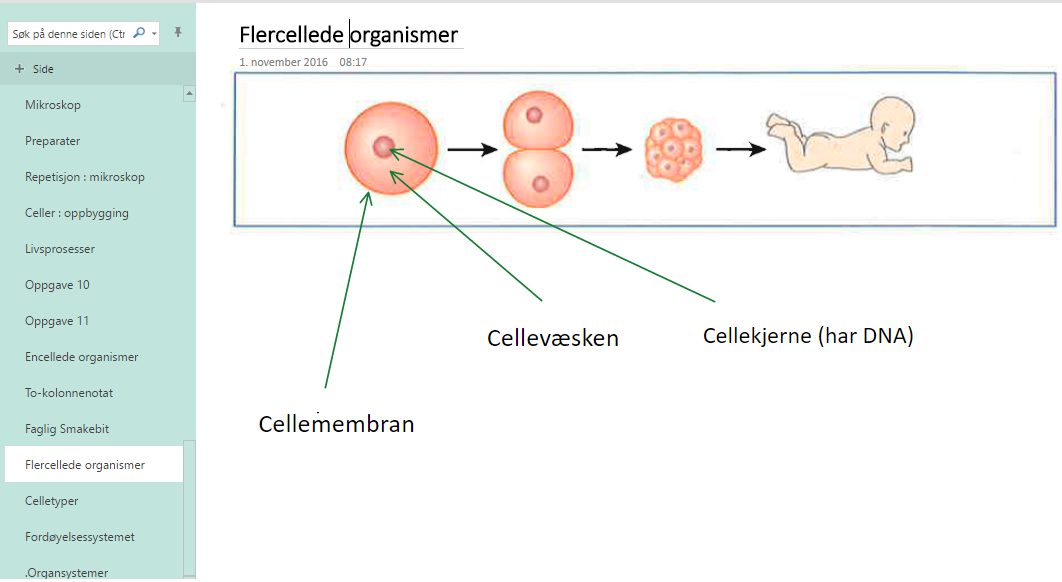
\includegraphics[scale = 0.6]{../figures/onenote_flercellet.png}
\caption{notat 1}
\label{fig:notat1}
\end{figure}

\begin{figure}[h!]
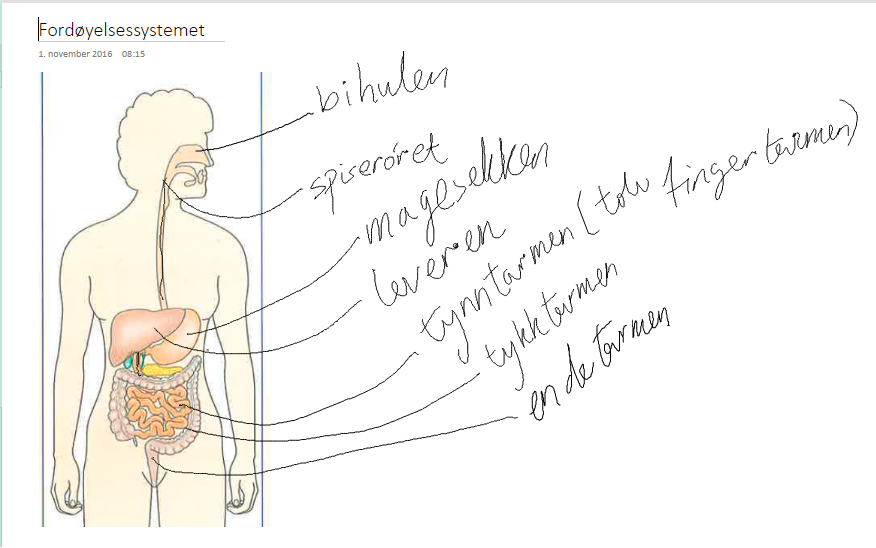
\includegraphics[scale = 0.6]{../figures/onenote_fordoyelse.png}
\caption{notat 2}
\label{fig:notat2}
\end{figure}

\subsection*{1.time}

Hensikten med denne timen er å oppsumere det elevene har lært hittil om celler og 
levendeorganismer, og innføre et nytt tema om encellede organismer. Timen starter med repetisjon 
av det elevene har lært fra tidligere timer, deriblant om mikroskop og cellestruktur. Ved oppstart 
av timen initierer vi elevene til å reflektere over temaer og begreper de har lært -og hatt lekser 
om. Vi bruker IRE/F metoden til å spørre blant elevene som rekker opp hånda. Det viser seg at det 
er noen få elever, som viser trygghet og kontroll når de responderer til lærer initiert dialog. 

En av de viktigste egenskapene en lærer kan utvise er evnen til å tilpasse seg i forhold til 
klassen, en gruppe og på individ nivå. Ved å erkjenne at alle elevene skal ha kjennskap til 
begrepene som blir tatt opp og repetert, er det da nødvendig å få bekreftet at elevene innehar en 
overordnet forståelse. Det kan derfor være nødvendig å frempeke noen elever som ikke viser aktiv 
deltagelse i timen og frembringe deres respons. Derimot er dette problematisk hvis det viser seg at 
de ikke har forutsetninger til å kunne respondere. Da settes de i en vanskelig situasjon hvor det 
blir nødvendig for læreren å lede de ut, ved hjelp av for eksempel ledende spørsmål. Derimot hvis 
det er forventet at det er en del av forutsetningene at elevene skal kunne respondere til lærer 
initiativ, da kan utspørringen av elevene frembringe kunnskap om deres hull. I neste time blir en 
annen form for lærer initiativ brukt til å frembringe respons. 
 
Siden elevene gjennom heleklassesamtalen har blitt "varmet" opp kognitivt, er de mottagelige for å 
et nytt tema. Innføringen av nytt tema er bevisst satt opp på en slik måte at overgangen fra 
repetisjon blir naturlig og flyttende. Hensikten er å la elevene danne et helhetlig bilde om
celler. I timene hvor de har hatt en innføring om celler, har de lært om basale strukturer.
I denne timen går de litt dypere ved å få en innføring om en av klassifikasjonene av celler.
Hensikten med innføringen er todelt : gjøre elevene bevisst om at det finnes forskjellige typer
celler, og gjøre de klar for den siste timen hvor de vil studere slike type celler under mikroskop.

Siden det er til hensikt å bruke resterende del av timen til repetisjon, var det ikke nødvendig å 
prøve å finne svakheter i elevenes respons gjennom helklassesamtalen. For å finne slike svakheter 
ble gruppesamtalene en bedre plattform. I den forbindelse ble tokolonnenotatet tatt i bruk (se 
vedlegg : \ref{sec:tokolonnenotat}). Hensikten med denne øvelsen er å la elevene jobbe sammen
i grupper om samme tema, hvor de blir enige med hverandre om hva som er viktig å være klar over
for deres utdelte temaer og begreper. Deretter ble de fordelt i nye grupper slik at hver 
gruppe hadde minst en elev som hadde forbredt sitt tema. Under hele denne prosessen var vi
tilgjengelige til å gå rundt å høre elevene diskutere begreper først sammen i grupper, og deretter
individuelt når de fremfører sine konklusjoner med medelever. Hvis vi merket at eleven hadde
problemmer med å gi tilstrekkelig respons om en gitt tema, initierte vi eleven i en dialog hvor
vi forsøkte å konstruere sammen en mer utdypet forståelse om begrepene. 

\subsection*{2.time}

Timen starter igjen på tilsvarende vis som den første timen. Derimot i denne timen er oppsettet 
forskjellig. Hensikten med timen er å repetere leksene elevene har fått til timen, om celletyper og
utvikling av celler fra enkeltceller til flercelledeorganismer. Etter å konsultert med vår veileder 
var vi nå klar over at alle elevene hadde forutsetninger til å kunne respondere til våre spørsmål, 
så lenge de var relatert til leksene. Etter den første timen var vi nå bevisste på at elevenes 
respons var avhengig av deres trygghet med en gitt tema. Vi valgte derfor å bruke navnekort 
isteden, hvor en elevs navn ble opplest vilkårlig fra en usortert liste, og deretter fikk eleven 
ordet og tid til å respondere.

\subsection*{3.time}

\end{document}
